\documentclass[]{book}
\usepackage{lmodern}
\usepackage{amssymb,amsmath}
\usepackage{ifxetex,ifluatex}
\usepackage{fixltx2e} % provides \textsubscript
\ifnum 0\ifxetex 1\fi\ifluatex 1\fi=0 % if pdftex
  \usepackage[T1]{fontenc}
  \usepackage[utf8]{inputenc}
\else % if luatex or xelatex
  \ifxetex
    \usepackage{mathspec}
  \else
    \usepackage{fontspec}
  \fi
  \defaultfontfeatures{Ligatures=TeX,Scale=MatchLowercase}
\fi
% use upquote if available, for straight quotes in verbatim environments
\IfFileExists{upquote.sty}{\usepackage{upquote}}{}
% use microtype if available
\IfFileExists{microtype.sty}{%
\usepackage{microtype}
\UseMicrotypeSet[protrusion]{basicmath} % disable protrusion for tt fonts
}{}
\usepackage[margin=1in]{geometry}
\usepackage{hyperref}
\hypersetup{unicode=true,
            pdftitle={YaRrr! The Pirate's Guide to R},
            pdfauthor={Nathaniel D. Phillips},
            pdfborder={0 0 0},
            breaklinks=true}
\urlstyle{same}  % don't use monospace font for urls
\usepackage{natbib}
\bibliographystyle{apalike}
\usepackage{color}
\usepackage{fancyvrb}
\newcommand{\VerbBar}{|}
\newcommand{\VERB}{\Verb[commandchars=\\\{\}]}
\DefineVerbatimEnvironment{Highlighting}{Verbatim}{commandchars=\\\{\}}
% Add ',fontsize=\small' for more characters per line
\usepackage{framed}
\definecolor{shadecolor}{RGB}{248,248,248}
\newenvironment{Shaded}{\begin{snugshade}}{\end{snugshade}}
\newcommand{\KeywordTok}[1]{\textcolor[rgb]{0.13,0.29,0.53}{\textbf{{#1}}}}
\newcommand{\DataTypeTok}[1]{\textcolor[rgb]{0.13,0.29,0.53}{{#1}}}
\newcommand{\DecValTok}[1]{\textcolor[rgb]{0.00,0.00,0.81}{{#1}}}
\newcommand{\BaseNTok}[1]{\textcolor[rgb]{0.00,0.00,0.81}{{#1}}}
\newcommand{\FloatTok}[1]{\textcolor[rgb]{0.00,0.00,0.81}{{#1}}}
\newcommand{\ConstantTok}[1]{\textcolor[rgb]{0.00,0.00,0.00}{{#1}}}
\newcommand{\CharTok}[1]{\textcolor[rgb]{0.31,0.60,0.02}{{#1}}}
\newcommand{\SpecialCharTok}[1]{\textcolor[rgb]{0.00,0.00,0.00}{{#1}}}
\newcommand{\StringTok}[1]{\textcolor[rgb]{0.31,0.60,0.02}{{#1}}}
\newcommand{\VerbatimStringTok}[1]{\textcolor[rgb]{0.31,0.60,0.02}{{#1}}}
\newcommand{\SpecialStringTok}[1]{\textcolor[rgb]{0.31,0.60,0.02}{{#1}}}
\newcommand{\ImportTok}[1]{{#1}}
\newcommand{\CommentTok}[1]{\textcolor[rgb]{0.56,0.35,0.01}{\textit{{#1}}}}
\newcommand{\DocumentationTok}[1]{\textcolor[rgb]{0.56,0.35,0.01}{\textbf{\textit{{#1}}}}}
\newcommand{\AnnotationTok}[1]{\textcolor[rgb]{0.56,0.35,0.01}{\textbf{\textit{{#1}}}}}
\newcommand{\CommentVarTok}[1]{\textcolor[rgb]{0.56,0.35,0.01}{\textbf{\textit{{#1}}}}}
\newcommand{\OtherTok}[1]{\textcolor[rgb]{0.56,0.35,0.01}{{#1}}}
\newcommand{\FunctionTok}[1]{\textcolor[rgb]{0.00,0.00,0.00}{{#1}}}
\newcommand{\VariableTok}[1]{\textcolor[rgb]{0.00,0.00,0.00}{{#1}}}
\newcommand{\ControlFlowTok}[1]{\textcolor[rgb]{0.13,0.29,0.53}{\textbf{{#1}}}}
\newcommand{\OperatorTok}[1]{\textcolor[rgb]{0.81,0.36,0.00}{\textbf{{#1}}}}
\newcommand{\BuiltInTok}[1]{{#1}}
\newcommand{\ExtensionTok}[1]{{#1}}
\newcommand{\PreprocessorTok}[1]{\textcolor[rgb]{0.56,0.35,0.01}{\textit{{#1}}}}
\newcommand{\AttributeTok}[1]{\textcolor[rgb]{0.77,0.63,0.00}{{#1}}}
\newcommand{\RegionMarkerTok}[1]{{#1}}
\newcommand{\InformationTok}[1]{\textcolor[rgb]{0.56,0.35,0.01}{\textbf{\textit{{#1}}}}}
\newcommand{\WarningTok}[1]{\textcolor[rgb]{0.56,0.35,0.01}{\textbf{\textit{{#1}}}}}
\newcommand{\AlertTok}[1]{\textcolor[rgb]{0.94,0.16,0.16}{{#1}}}
\newcommand{\ErrorTok}[1]{\textcolor[rgb]{0.64,0.00,0.00}{\textbf{{#1}}}}
\newcommand{\NormalTok}[1]{{#1}}
\usepackage{longtable,booktabs}
\usepackage{graphicx,grffile}
\makeatletter
\def\maxwidth{\ifdim\Gin@nat@width>\linewidth\linewidth\else\Gin@nat@width\fi}
\def\maxheight{\ifdim\Gin@nat@height>\textheight\textheight\else\Gin@nat@height\fi}
\makeatother
% Scale images if necessary, so that they will not overflow the page
% margins by default, and it is still possible to overwrite the defaults
% using explicit options in \includegraphics[width, height, ...]{}
\setkeys{Gin}{width=\maxwidth,height=\maxheight,keepaspectratio}
\IfFileExists{parskip.sty}{%
\usepackage{parskip}
}{% else
\setlength{\parindent}{0pt}
\setlength{\parskip}{6pt plus 2pt minus 1pt}
}
\setlength{\emergencystretch}{3em}  % prevent overfull lines
\providecommand{\tightlist}{%
  \setlength{\itemsep}{0pt}\setlength{\parskip}{0pt}}
\setcounter{secnumdepth}{5}
% Redefines (sub)paragraphs to behave more like sections
\ifx\paragraph\undefined\else
\let\oldparagraph\paragraph
\renewcommand{\paragraph}[1]{\oldparagraph{#1}\mbox{}}
\fi
\ifx\subparagraph\undefined\else
\let\oldsubparagraph\subparagraph
\renewcommand{\subparagraph}[1]{\oldsubparagraph{#1}\mbox{}}
\fi

%%% Use protect on footnotes to avoid problems with footnotes in titles
\let\rmarkdownfootnote\footnote%
\def\footnote{\protect\rmarkdownfootnote}

%%% Change title format to be more compact
\usepackage{titling}

% Create subtitle command for use in maketitle
\newcommand{\subtitle}[1]{
  \posttitle{
    \begin{center}\large#1\end{center}
    }
}

\setlength{\droptitle}{-2em}
  \title{YaRrr! The Pirate's Guide to R}
  \pretitle{\vspace{\droptitle}\centering\huge}
  \posttitle{\par}
  \author{Nathaniel D. Phillips}
  \preauthor{\centering\large\emph}
  \postauthor{\par}
  \predate{\centering\large\emph}
  \postdate{\par}
  \date{2017-02-27}

\usepackage{booktabs}
\usepackage{amsthm}
\makeatletter
\def\thm@space@setup{%
  \thm@preskip=8pt plus 2pt minus 4pt
  \thm@postskip=\thm@preskip
}
\makeatother

\usepackage{amsthm}
\newtheorem{theorem}{Theorem}[chapter]
\newtheorem{lemma}{Lemma}[chapter]
\theoremstyle{definition}
\newtheorem{definition}{Definition}[chapter]
\newtheorem{corollary}{Corollary}[chapter]
\newtheorem{proposition}{Proposition}[chapter]
\theoremstyle{definition}
\newtheorem{example}{Example}[chapter]
\theoremstyle{remark}
\newtheorem*{remark}{Remark}
\begin{document}
\maketitle

{
\setcounter{tocdepth}{1}
\tableofcontents
}
\chapter{Preface}\label{intro}

\chapter{Getting Started}\label{started}

\chapter{Jump In!}\label{jumpin}

\chapter{The Basics}\label{basics}

\chapter{Scalers and vectors}\label{scalersvectors}

\chapter{Vector functions}\label{vectorfunctions}

\chapter{Indexing Vectors with {[} {]}}\label{vectorindexing}

\begin{figure}

{\centering 
\includegraphics[width=0.5\linewidth]{images/antiqueboat} 

}

\end{figure}

\begin{tabular}{l|l|r|r|r}
\hline
boat.names & boat.colors & boat.ages & boat.prices & boat.costs\\
\hline
a & black & 143 & 53 & 52\\
\hline
b & green & 53 & 87 & 80\\
\hline
c & pink & 356 & 54 & 20\\
\hline
d & blue & 23 & 66 & 100\\
\hline
e & blue & 647 & 264 & 189\\
\hline
f & green & 24 & 32 & 12\\
\hline
g & green & 532 & 532 & 520\\
\hline
h & yellow & 43 & 58 & 68\\
\hline
i & black & 66 & 99 & 80\\
\hline
j & black & 86 & 132 & 100\\
\hline
\end{tabular}

\begin{Shaded}
\begin{Highlighting}[]
\CommentTok{# Boat sale. Creating the data vectors}
\NormalTok{boat.names <-}\StringTok{ }\KeywordTok{c}\NormalTok{(}\StringTok{"a"}\NormalTok{, }\StringTok{"b"}\NormalTok{, }\StringTok{"c"}\NormalTok{, }\StringTok{"d"}\NormalTok{, }\StringTok{"e"}\NormalTok{, }\StringTok{"f"}\NormalTok{, }\StringTok{"g"}\NormalTok{, }\StringTok{"h"}\NormalTok{, }\StringTok{"i"}\NormalTok{, }\StringTok{"j"}\NormalTok{)}
\NormalTok{boat.colors <-}\StringTok{ }\KeywordTok{c}\NormalTok{(}\StringTok{"black"}\NormalTok{, }\StringTok{"green"}\NormalTok{, }\StringTok{"pink"}\NormalTok{, }\StringTok{"blue"}\NormalTok{, }\StringTok{"blue"}\NormalTok{, }
                \StringTok{"green"}\NormalTok{, }\StringTok{"green"}\NormalTok{, }\StringTok{"yellow"}\NormalTok{, }\StringTok{"black"}\NormalTok{, }\StringTok{"black"}\NormalTok{)}
\NormalTok{boat.ages <-}\StringTok{ }\KeywordTok{c}\NormalTok{(}\DecValTok{143}\NormalTok{, }\DecValTok{53}\NormalTok{, }\DecValTok{356}\NormalTok{, }\DecValTok{23}\NormalTok{, }\DecValTok{647}\NormalTok{, }\DecValTok{24}\NormalTok{, }\DecValTok{532}\NormalTok{, }\DecValTok{43}\NormalTok{, }\DecValTok{66}\NormalTok{, }\DecValTok{86}\NormalTok{)}
\NormalTok{boat.prices <-}\StringTok{ }\KeywordTok{c}\NormalTok{(}\DecValTok{53}\NormalTok{, }\DecValTok{87}\NormalTok{, }\DecValTok{54}\NormalTok{, }\DecValTok{66}\NormalTok{, }\DecValTok{264}\NormalTok{, }\DecValTok{32}\NormalTok{, }\DecValTok{532}\NormalTok{, }\DecValTok{58}\NormalTok{, }\DecValTok{99}\NormalTok{, }\DecValTok{132}\NormalTok{)}
\NormalTok{boat.costs <-}\StringTok{ }\KeywordTok{c}\NormalTok{(}\DecValTok{52}\NormalTok{, }\DecValTok{80}\NormalTok{, }\DecValTok{20}\NormalTok{, }\DecValTok{100}\NormalTok{, }\DecValTok{189}\NormalTok{, }\DecValTok{12}\NormalTok{, }\DecValTok{520}\NormalTok{, }\DecValTok{68}\NormalTok{, }\DecValTok{80}\NormalTok{, }\DecValTok{100}\NormalTok{)}

\CommentTok{# What was the price of the first boat?}
\NormalTok{boat.prices[}\DecValTok{1}\NormalTok{]}
\NormalTok{## [1] 53}

\CommentTok{# What were the ages of the first 5 boats?}
\NormalTok{boat.ages[}\DecValTok{1}\NormalTok{:}\DecValTok{5}\NormalTok{]}
\NormalTok{## [1] 143  53 356  23 647}

\CommentTok{# What were the names of the black boats?}
\NormalTok{boat.names[boat.colors ==}\StringTok{ "black"}\NormalTok{]}
\NormalTok{## [1] "a" "i" "j"}

\CommentTok{# What were the prices of either green or yellow boats?}
\NormalTok{boat.prices[boat.colors ==}\StringTok{ "green"} \NormalTok{|}\StringTok{ }\NormalTok{boat.colors ==}\StringTok{ "yellow"}\NormalTok{]}
\NormalTok{## [1]  87  32 532  58}

\CommentTok{# Change the price of boat "s" to 100}
\NormalTok{boat.prices[boat.names ==}\StringTok{ "s"}\NormalTok{] <-}\StringTok{ }\DecValTok{100}

\CommentTok{# What was the median price of black boats less than 100 years old?}
\KeywordTok{median}\NormalTok{(boat.prices[boat.colors ==}\StringTok{ "black"} \NormalTok{&}\StringTok{ }\NormalTok{boat.ages <}\StringTok{ }\DecValTok{100}\NormalTok{])}
\NormalTok{## [1] 115.5}

\CommentTok{# How many pink boats were there?}
\KeywordTok{sum}\NormalTok{(boat.colors ==}\StringTok{ "pink"}\NormalTok{)}
\NormalTok{## [1] 1}

\CommentTok{# What percent of boats were older than 100 years old?}
\KeywordTok{mean}\NormalTok{(boat.ages <}\StringTok{ }\DecValTok{100}\NormalTok{)}
\NormalTok{## [1] 0.6}
\end{Highlighting}
\end{Shaded}

By now you should be a whiz at applying functions like \texttt{mean()}
and \texttt{table()} to vectors. However, in many analyses, you won't
want to calculate statistics of an entire vector. Instead, you will want
to access specific \emph{subsets} of values of a vector based on some
criteria. For example, you may want to access values in a specific
location in the vector (i.e.; the first 10 elements) or based on some
criteria within that vector (i.e.; all values greater than 0), or based
on criterion from values in a \emph{different} vector (e.g.; All values
of age where sex is Female). To access specific values of a vector in R,
we use \emph{indexing} using brackets \texttt{{[}{]}}. In general,
whatever you put inside the brackets, tells R which values of the vector
object you want. There are two main ways that you can use indexing to
access subsets of data in a vector: numerical and logical indexing.

\section{Numerical Indexing}\label{numerical-indexing}

With numerical indexing, you enter a vector of integers corresponding to
the values in the vector you want to access in the form
\texttt{a{[}index{]}}, where \texttt{a} is the vector, and
\texttt{index} is a vector of index values. For example, let's use
numerical indexing to get values from our boat vectors.

\begin{Shaded}
\begin{Highlighting}[]
\CommentTok{# What is the first boat name?}
\NormalTok{boat.names[}\DecValTok{1}\NormalTok{]}
\NormalTok{## [1] "a"}

\CommentTok{# What are the first five boat colors?}
\NormalTok{boat.colors[}\DecValTok{1}\NormalTok{:}\DecValTok{5}\NormalTok{]}
\NormalTok{## [1] "black" "green" "pink"  "blue"  "blue"}

\CommentTok{# What is every second boat age?}
\NormalTok{boat.ages[}\KeywordTok{seq}\NormalTok{(}\DecValTok{1}\NormalTok{, }\DecValTok{5}\NormalTok{, }\DataTypeTok{by =} \DecValTok{2}\NormalTok{)]}
\NormalTok{## [1] 143 356 647}
\end{Highlighting}
\end{Shaded}

You can use any indexing vector as long as it contains integers. You can
even access the same elements multiple times:

\begin{Shaded}
\begin{Highlighting}[]
\CommentTok{# What is the first boat age (3 times)}
\NormalTok{boat.ages[}\KeywordTok{c}\NormalTok{(}\DecValTok{1}\NormalTok{, }\DecValTok{1}\NormalTok{, }\DecValTok{1}\NormalTok{)]}
\NormalTok{## [1] 143 143 143}
\end{Highlighting}
\end{Shaded}

It it makes your code clearer, you can define an indexing object before
doing your actual indexing. For example, let's define an object called
\texttt{my.index} and use this object to index our data vector:

\begin{Shaded}
\begin{Highlighting}[]
\NormalTok{my.index <-}\StringTok{ }\DecValTok{3}\NormalTok{:}\DecValTok{5}
\NormalTok{boat.names[my.index]}
\NormalTok{## [1] "c" "d" "e"}
\end{Highlighting}
\end{Shaded}

\section{Logical Indexing}\label{logical-indexing}

\begin{figure}

{\centering 
\includegraphics[width=0.5\linewidth]{images/logic} 

}

\caption{Logical indexing. Good for R aliens and R pirates.}\label{fig:unnamed-chunk-8}
\end{figure}

The second way to index vectors is with \emph{logical vectors}. A
logical vector is a vector that \emph{only} contains TRUE and FALSE
values. In R, true values are designated with TRUE, and false values
with FALSE. When you index a vector with a logical vector, R will return
values of the vector for which the indexing vector is TRUE. If that was
confusing, think about it this way: a logical vector, combined with the
brackets \texttt{{[}\ {]}}, acts as a \emph{filter} for the vector it is
indexing. It only lets values of the vector pass through for which the
logical vector is TRUE.

\begin{figure}

{\centering 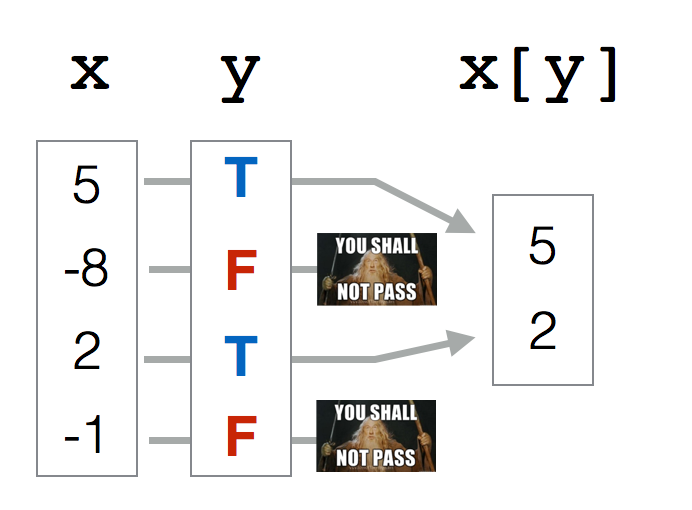
\includegraphics[width=0.5\linewidth]{images/indexgandolf} 

}

\caption{FALSE values in a logical vector are like lots of mini-Gandolfs. In this example, I am indexing a vector x with a logical vector y (y for example could be x > 0, so all positive values of x are TRUE and all negative values are FALSE). The result is a vector of length 2, which are the values of x for which the logical vector y was true. Gandolf stopped all the values of x for which y was FALSE.}\label{fig:unnamed-chunk-9}
\end{figure}

You could create logical vectors directly using \texttt{c()}. For
example, I could access every other value of the following vector as
follows:

\begin{Shaded}
\begin{Highlighting}[]
\NormalTok{a <-}\StringTok{ }\KeywordTok{c}\NormalTok{(}\DecValTok{1}\NormalTok{, }\DecValTok{2}\NormalTok{, }\DecValTok{3}\NormalTok{, }\DecValTok{4}\NormalTok{, }\DecValTok{5}\NormalTok{)}
\NormalTok{a[}\KeywordTok{c}\NormalTok{(}\OtherTok{TRUE}\NormalTok{, }\OtherTok{FALSE}\NormalTok{, }\OtherTok{TRUE}\NormalTok{, }\OtherTok{FALSE}\NormalTok{, }\OtherTok{TRUE}\NormalTok{)]}
\NormalTok{## [1] 1 3 5}
\end{Highlighting}
\end{Shaded}

As you can see, R returns all values of the vector \texttt{a} for which
the logical vector is TRUE.

\begin{figure}[htbp]
\centering
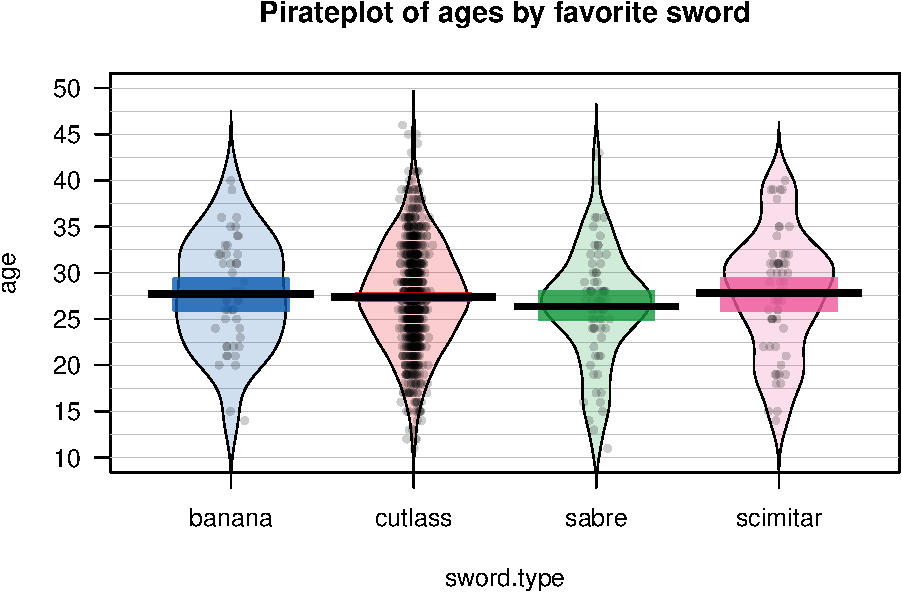
\includegraphics{YaRrr_files/figure-latex/unnamed-chunk-11-1.pdf}
\caption{\label{fig:unnamed-chunk-11}Logical comparison operators in R}
\end{figure}

However, creating logical vectors using \texttt{c()} is tedious.
Instead, it's better to create logical vectors from \emph{existing
vectors} using comparison operators like \textless{} (less than), ==
(equals to), and != (not equal to). A complete list of the most common
comparison operators is in Figure\textasciitilde{}\ref{fig:comparison}.
For example, let's create some logical vectors from our
\texttt{boat.ages} vector:

\begin{Shaded}
\begin{Highlighting}[]
\CommentTok{# Which ages are > 100?}
\NormalTok{boat.ages >}\StringTok{ }\DecValTok{100}
\NormalTok{##  [1]  TRUE FALSE  TRUE FALSE  TRUE FALSE  TRUE FALSE FALSE FALSE}

\CommentTok{# Which ages are equal to 23?}
\NormalTok{boat.ages ==}\StringTok{ }\DecValTok{23}
\NormalTok{##  [1] FALSE FALSE FALSE  TRUE FALSE FALSE FALSE FALSE FALSE FALSE}

\CommentTok{# Which boat names are equal to c?}
\NormalTok{boat.names ==}\StringTok{ "c"}
\NormalTok{##  [1] FALSE FALSE  TRUE FALSE FALSE FALSE FALSE FALSE FALSE FALSE}
\end{Highlighting}
\end{Shaded}

You can also create logical vectors by comparing a vector to another
vector of the same length. When you do this, R will compare values in
the same position (e.g.; the first values will be compared, then the
second values, etc.). For example, we can compare the \texttt{boat.cost}
and \texttt{boat.price} vectors to see which boats sold for a higher
price than their cost:

\begin{Shaded}
\begin{Highlighting}[]
\CommentTok{# Which boats had a higher price than cost?}
\NormalTok{boat.prices >}\StringTok{ }\NormalTok{boat.costs}
\NormalTok{##  [1]  TRUE  TRUE  TRUE FALSE  TRUE  TRUE  TRUE FALSE  TRUE  TRUE}

\CommentTok{# Which boats had a lower price than cost?}
\NormalTok{boat.prices <}\StringTok{ }\NormalTok{boat.costs}
\NormalTok{##  [1] FALSE FALSE FALSE  TRUE FALSE FALSE FALSE  TRUE FALSE FALSE}
\end{Highlighting}
\end{Shaded}

Once you've created a logical vector using a comparison operator, you
can use it to index any vector with the same length. Here, I'll use
logical vectors to get the prices of boats whose ages were greater than
100:

\begin{Shaded}
\begin{Highlighting}[]
\CommentTok{# What were the prices of boats older than 100?}
\NormalTok{boat.prices[boat.ages >}\StringTok{ }\DecValTok{100}\NormalTok{]}
\NormalTok{## [1]  53  54 264 532}
\end{Highlighting}
\end{Shaded}

Here's how logical indexing works step-by-step:

\begin{Shaded}
\begin{Highlighting}[]
\CommentTok{# Which boat prices are greater than 100?}
\NormalTok{boat.ages >}\StringTok{ }\DecValTok{100}
\NormalTok{##  [1]  TRUE FALSE  TRUE FALSE  TRUE FALSE  TRUE FALSE FALSE FALSE}

\CommentTok{# Writing the logical index by hand (you'd never do this!)}
\NormalTok{boat.prices[}\KeywordTok{c}\NormalTok{(}\OtherTok{TRUE}\NormalTok{, }\OtherTok{FALSE}\NormalTok{, }\OtherTok{TRUE}\NormalTok{, }\OtherTok{FALSE}\NormalTok{, }\OtherTok{TRUE}\NormalTok{, }\OtherTok{FALSE}\NormalTok{, }\OtherTok{TRUE}\NormalTok{, }\OtherTok{FALSE}\NormalTok{, }\OtherTok{FALSE}\NormalTok{, }\OtherTok{FALSE}\NormalTok{)]}
\NormalTok{## [1]  53  54 264 532}

\CommentTok{# Doing it all in one step! You get the same answer}
\NormalTok{boat.prices[boat.ages >}\StringTok{ }\DecValTok{100}\NormalTok{]}
\NormalTok{## [1]  53  54 264 532}
\end{Highlighting}
\end{Shaded}

\subsection{\texorpdfstring{\texttt{\&} (and), \texttt{\textbar{}} (or),
\texttt{\%in\%}}{\& (and), \textbar{} (or), \%in\%}}\label{and-or-in}

In addition to using single comparison operators, you can combine
multiple logical vectors using the OR (which looks like
\texttt{\textbar{}} and AND \texttt{\textbackslash{}\&} commands. The OR
\texttt{\textbar{}} operation will return TRUE if any of the logical
vectors is TRUE, while the AND \texttt{\&} operation will only return
TRUE if all of the values in the logical vectors is TRUE. This is
especially powerful when you want to create a logical vector based on
criteria from multiple vectors.

For example, let's create a logical vector indicating which boats had a
price greater than 200 OR less than 100, and then use that vector to see
what the names of these boats were:

\begin{Shaded}
\begin{Highlighting}[]
\CommentTok{# Which boats had prices greater than 400 OR less than 100?}
\NormalTok{boat.prices >}\StringTok{ }\DecValTok{200} \NormalTok{|}\StringTok{ }\NormalTok{boat.prices <}\StringTok{ }\DecValTok{100}
\NormalTok{##  [1]  TRUE  TRUE  TRUE  TRUE  TRUE  TRUE  TRUE  TRUE  TRUE FALSE}

\CommentTok{# What were the NAMES of these boats}
\NormalTok{boat.names[boat.prices >}\StringTok{ }\DecValTok{200} \NormalTok{|}\StringTok{ }\NormalTok{boat.prices <}\StringTok{ }\DecValTok{100}\NormalTok{]}
\NormalTok{## [1] "a" "b" "c" "d" "e" "f" "g" "h" "i"}
\end{Highlighting}
\end{Shaded}

You can combine as many logical vectors as you want (as long as they all
have the same length!):

\begin{Shaded}
\begin{Highlighting}[]
\CommentTok{# Boat names of boats with a color of black OR with a price > 100}
\NormalTok{boat.names[boat.colors ==}\StringTok{ "black"} \NormalTok{|}\StringTok{ }\NormalTok{boat.prices >}\StringTok{ }\DecValTok{100}\NormalTok{]}
\NormalTok{## [1] "a" "e" "g" "i" "j"}

\CommentTok{# Names of blue boats with a price greater than 200}
\NormalTok{boat.names[boat.colors ==}\StringTok{ "blue"} \NormalTok{&}\StringTok{ }\NormalTok{boat.prices >}\StringTok{ }\DecValTok{200}\NormalTok{]}
\NormalTok{## [1] "e"}
\end{Highlighting}
\end{Shaded}

You can combine as many logical vectors as you want to create
increasingly complex selection criteria. For example, the following
logical vector returns TRUE for cases where the boat colors are black OR
brown, AND where the price was not equal to 100:

\begin{Shaded}
\begin{Highlighting}[]
\CommentTok{# Which boats were eithe black or brown, AND had a price less than 100?}
\NormalTok{(boat.colors ==}\StringTok{ "black"} \NormalTok{|}\StringTok{ }\NormalTok{boat.colors ==}\StringTok{ "brown"}\NormalTok{) &}\StringTok{ }\NormalTok{boat.prices <}\StringTok{ }\DecValTok{100}
\NormalTok{##  [1]  TRUE FALSE FALSE FALSE FALSE FALSE FALSE FALSE  TRUE FALSE}

\CommentTok{# What were the names of these boats?}
\NormalTok{boat.names[(boat.colors ==}\StringTok{ "black"} \NormalTok{|}\StringTok{ }\NormalTok{boat.colors ==}\StringTok{ "brown"}\NormalTok{) &}\StringTok{ }\NormalTok{boat.prices <}\StringTok{ }\DecValTok{100}\NormalTok{]}
\NormalTok{## [1] "a" "i"}
\end{Highlighting}
\end{Shaded}

When using multiple criteria, make sure to use parentheses when
appropriate. If I didn't use parentheses above, I would get a different
answer.

The \texttt{\%in\%} operation helps you to easily create multiple OR
arguments.Imagine you have a vector of categorical data that can take on
many different values. For example, you could have a vector x indicating
people's favorite letters.

\begin{Shaded}
\begin{Highlighting}[]
\NormalTok{x <-}\StringTok{ }\KeywordTok{c}\NormalTok{(}\StringTok{"a"}\NormalTok{, }\StringTok{"t"}\NormalTok{, }\StringTok{"a"}\NormalTok{, }\StringTok{"b"}\NormalTok{, }\StringTok{"z"}\NormalTok{)}
\end{Highlighting}
\end{Shaded}

Now, let's say you want to create a logical vector indicating which
values are either a or b or c or d. You could create this logical vector
with multiple \textbar{} (OR) commands:

\begin{Shaded}
\begin{Highlighting}[]
\NormalTok{x ==}\StringTok{ "a"} \NormalTok{|}\StringTok{ }\NormalTok{x ==}\StringTok{ "b"} \NormalTok{|}\StringTok{ }\NormalTok{x ==}\StringTok{ "c"} \NormalTok{|}\StringTok{ }\NormalTok{x ==}\StringTok{ "d"}
\NormalTok{## [1]  TRUE FALSE  TRUE  TRUE FALSE}
\end{Highlighting}
\end{Shaded}

However, this takes a long time to write. Thankfully, the
\texttt{\%in\%} operation allows you to combine multiple OR comparisons
much faster. To use the \texttt{\%in\%} function, just put it in between
the original vector, and a new vector of possible values. The
\texttt{\%in\%} function goes through every value in the vector x, and
returns TRUE if it finds it in the vector of possible values --
otherwise it returns FALSE.

\begin{Shaded}
\begin{Highlighting}[]
\NormalTok{x %in%}\StringTok{ }\KeywordTok{c}\NormalTok{(}\StringTok{"a"}\NormalTok{, }\StringTok{"b"}\NormalTok{, }\StringTok{"c"}\NormalTok{, }\StringTok{"d"}\NormalTok{)}
\NormalTok{## [1]  TRUE FALSE  TRUE  TRUE FALSE}
\end{Highlighting}
\end{Shaded}

As you can see, the result is identical to our previous result.

\subsection{Counts and percentages from logical
vectors}\label{counts-and-percentages-from-logical-vectors}

Many (if not all) R functions will interpret TRUE values as 1 and FALSE
values as 0. This allows us to easily answer questions like ``How many
values in a data vector are greater than 0?'' or ``What percentage of
values are equal to 5?'' by applying the \texttt{sum()} or
\texttt{mean()} function to a logical vector.

We'll start with a vector x of length 10, containing 3 positive numbers
and 5 negative numbers.

\begin{Shaded}
\begin{Highlighting}[]
\NormalTok{x <-}\StringTok{ }\KeywordTok{c}\NormalTok{(}\DecValTok{1}\NormalTok{, }\DecValTok{2}\NormalTok{, }\DecValTok{3}\NormalTok{, -}\DecValTok{5}\NormalTok{, -}\DecValTok{5}\NormalTok{, -}\DecValTok{5}\NormalTok{, -}\DecValTok{5}\NormalTok{, -}\DecValTok{5}\NormalTok{)}
\end{Highlighting}
\end{Shaded}

We can create a logical vector to see which values are greater than 0:

\begin{Shaded}
\begin{Highlighting}[]
\NormalTok{x >}\StringTok{ }\DecValTok{0}
\NormalTok{## [1]  TRUE  TRUE  TRUE FALSE FALSE FALSE FALSE FALSE}
\end{Highlighting}
\end{Shaded}

Now, we'll use \texttt{sum()} and \texttt{mean()} on that logical vector
to see how many of the values in x are positive, and what percent are
positive. We should find that there are 5 TRUE values, and that 50\% of
the values (5 / 10) are TRUE.

\begin{Shaded}
\begin{Highlighting}[]
\KeywordTok{sum}\NormalTok{(x >}\StringTok{ }\DecValTok{0}\NormalTok{)}
\NormalTok{## [1] 3}
\KeywordTok{mean}\NormalTok{(x >}\StringTok{ }\DecValTok{0}\NormalTok{)}
\NormalTok{## [1] 0.375}
\end{Highlighting}
\end{Shaded}

This is a \emph{really} powerful tool. Pretty much \emph{any} time you
want to answer a question like ``How many of X are Y'' or ``What percent
of X are Y'', you use \texttt{sum()} or \texttt{mean()} function with a
logical vector as an argument.

\subsection{Additional Logical
functions}\label{additional-logical-functions}

R has lots of special functions that take vectors as arguments, and
return logical vectors based on multiple criteria. For example, you can
use the \texttt{is.na()} function to test which values of a vector are
missing. Table \ref{tab:logicalfunctions} contains some that I
frequently use:

\begin{longtable}[]{@{}llll@{}}
\caption{\label{tab:logicalfunctions} Functions to create and use logical
vectors.}\tabularnewline
\toprule
\begin{minipage}[b]{0.20\columnwidth}\raggedright\strut
Function\strut
\end{minipage} & \begin{minipage}[b]{0.23\columnwidth}\raggedright\strut
Description\strut
\end{minipage} & \begin{minipage}[b]{0.31\columnwidth}\raggedright\strut
Example\strut
\end{minipage} & \begin{minipage}[b]{0.06\columnwidth}\raggedright\strut
Result\strut
\end{minipage}\tabularnewline
\midrule
\endfirsthead
\toprule
\begin{minipage}[b]{0.20\columnwidth}\raggedright\strut
Function\strut
\end{minipage} & \begin{minipage}[b]{0.23\columnwidth}\raggedright\strut
Description\strut
\end{minipage} & \begin{minipage}[b]{0.31\columnwidth}\raggedright\strut
Example\strut
\end{minipage} & \begin{minipage}[b]{0.06\columnwidth}\raggedright\strut
Result\strut
\end{minipage}\tabularnewline
\midrule
\endhead
\begin{minipage}[t]{0.20\columnwidth}\raggedright\strut
\texttt{is.na(x)}\strut
\end{minipage} & \begin{minipage}[t]{0.23\columnwidth}\raggedright\strut
Which values in x are NA?\strut
\end{minipage} & \begin{minipage}[t]{0.31\columnwidth}\raggedright\strut
\texttt{is.na(c(2,\ NA,\ 5))}\strut
\end{minipage} & \begin{minipage}[t]{0.06\columnwidth}\raggedright\strut
FALSE, TRUE, FALSE\strut
\end{minipage}\tabularnewline
\begin{minipage}[t]{0.20\columnwidth}\raggedright\strut
\texttt{is.finite(x)}\strut
\end{minipage} & \begin{minipage}[t]{0.23\columnwidth}\raggedright\strut
Which values in x are numbers?\strut
\end{minipage} & \begin{minipage}[t]{0.31\columnwidth}\raggedright\strut
\texttt{is.finite(c(NA,\ 89,\ 0))}\strut
\end{minipage} & \begin{minipage}[t]{0.06\columnwidth}\raggedright\strut
FALSE, TRUE, TRUE\strut
\end{minipage}\tabularnewline
\begin{minipage}[t]{0.20\columnwidth}\raggedright\strut
\texttt{duplicated(x)}\strut
\end{minipage} & \begin{minipage}[t]{0.23\columnwidth}\raggedright\strut
Which values in x are duplicated?\strut
\end{minipage} & \begin{minipage}[t]{0.31\columnwidth}\raggedright\strut
\texttt{duplicated(c(1,\ 4,\ 1,\ 2))}\strut
\end{minipage} & \begin{minipage}[t]{0.06\columnwidth}\raggedright\strut
FALSE, FALSE, TRUE, FALSE\strut
\end{minipage}\tabularnewline
\begin{minipage}[t]{0.20\columnwidth}\raggedright\strut
\texttt{which(x)}\strut
\end{minipage} & \begin{minipage}[t]{0.23\columnwidth}\raggedright\strut
Which values in x are TRUE?\strut
\end{minipage} & \begin{minipage}[t]{0.31\columnwidth}\raggedright\strut
\texttt{which(c(TRUE,\ FALSE,\ TRUE))}\strut
\end{minipage} & \begin{minipage}[t]{0.06\columnwidth}\raggedright\strut
1, 3\strut
\end{minipage}\tabularnewline
\bottomrule
\end{longtable}

Logical vectors aren't just good for indexing, you can also use them to
figure out which values in a vector satisfy some criteria. To do this,
use the function \texttt{which()}. If you apply the function
\texttt{which()} to a logical vector, R will tell you which values of
the index are TRUE. For example:

\begin{Shaded}
\begin{Highlighting}[]
\CommentTok{# A vector of sex information}
\NormalTok{sex <-}\StringTok{ }\KeywordTok{c}\NormalTok{(}\StringTok{"m"}\NormalTok{, }\StringTok{"m"}\NormalTok{, }\StringTok{"f"}\NormalTok{, }\StringTok{"m"}\NormalTok{, }\StringTok{"f"}\NormalTok{, }\StringTok{"f"}\NormalTok{)}

\CommentTok{# Which values of sex are m?}
\KeywordTok{which}\NormalTok{(sex ==}\StringTok{ "m"}\NormalTok{)}
\NormalTok{## [1] 1 2 4}

\CommentTok{# Which values of sex are f?}
\KeywordTok{which}\NormalTok{(sex ==}\StringTok{ "f"}\NormalTok{)}
\NormalTok{## [1] 3 5 6}
\end{Highlighting}
\end{Shaded}

\section{Changing values of a vector}\label{changing-values-of-a-vector}

Now that you know how to index a vector, you can easily change specific
values in a vector using the assignment (\texttt{\textless{}-})
operation. To do this, just assign a vector of new values to the indexed
values of the original vector:

Let's create a vector \texttt{a} which contains 10 1s:

\begin{Shaded}
\begin{Highlighting}[]
\NormalTok{a <-}\StringTok{ }\KeywordTok{rep}\NormalTok{(}\DecValTok{1}\NormalTok{, }\DecValTok{10}\NormalTok{)}
\end{Highlighting}
\end{Shaded}

Now, let's change the first 5 values in the vector to 9s by indexing the
first five values, and assigning the value of 9:

\begin{Shaded}
\begin{Highlighting}[]
\NormalTok{a[}\DecValTok{1}\NormalTok{:}\DecValTok{5}\NormalTok{] <-}\StringTok{ }\DecValTok{9}
\NormalTok{a}
\NormalTok{##  [1] 9 9 9 9 9 1 1 1 1 1}
\end{Highlighting}
\end{Shaded}

Now let's change the last 5 values to 0s. We'll index the values 6
through 10, and assign a value of 0.

\begin{Shaded}
\begin{Highlighting}[]
\NormalTok{a[}\DecValTok{6}\NormalTok{:}\DecValTok{10}\NormalTok{] <-}\StringTok{ }\DecValTok{0}
\NormalTok{a}
\NormalTok{##  [1] 9 9 9 9 9 0 0 0 0 0}
\end{Highlighting}
\end{Shaded}

Of course, you can also change values of a vector using a logical
indexing vector. For example, let's say you have a vector of numbers
that should be from 1 to 10. If values are outside of this range, you
want to set them to either the minimum (1) or maximum (10) value:

\begin{Shaded}
\begin{Highlighting}[]
\CommentTok{# x is a vector of numbers that should be from 1 to 10}
\NormalTok{x <-}\StringTok{ }\KeywordTok{c}\NormalTok{(}\DecValTok{5}\NormalTok{, -}\DecValTok{5}\NormalTok{, }\DecValTok{7}\NormalTok{, }\DecValTok{4}\NormalTok{, }\DecValTok{11}\NormalTok{, }\DecValTok{5}\NormalTok{, -}\DecValTok{2}\NormalTok{)}

\CommentTok{# Assign values less than 1 to 1}
\NormalTok{x[x <}\StringTok{ }\DecValTok{1}\NormalTok{] <-}\StringTok{ }\DecValTok{1}

\CommentTok{# Assign values greater than 10 to 10}
\NormalTok{x[x >}\StringTok{ }\DecValTok{10}\NormalTok{] <-}\StringTok{ }\DecValTok{10}

\CommentTok{# Print the result!}
\NormalTok{x}
\NormalTok{## [1]  5  1  7  4 10  5  1}
\end{Highlighting}
\end{Shaded}

As you can see, our new values of x are now never less than 1 or greater
than 10!

\textbf{A note on indexing\ldots{}}

Technically, when you assign new values to a vector, you should always
assign a vector of the same length as the number of values that you are
updating. For example, given a vector a with 10 1s:

\begin{Shaded}
\begin{Highlighting}[]
\NormalTok{a <-}\StringTok{ }\KeywordTok{rep}\NormalTok{(}\DecValTok{1}\NormalTok{, }\DecValTok{10}\NormalTok{)}
\end{Highlighting}
\end{Shaded}

To update the first 5 values with 5 9s, we should assign a new vector of
5 9s

\begin{Shaded}
\begin{Highlighting}[]
\NormalTok{a[}\DecValTok{1}\NormalTok{:}\DecValTok{5}\NormalTok{] <-}\StringTok{ }\KeywordTok{c}\NormalTok{(}\DecValTok{9}\NormalTok{, }\DecValTok{9}\NormalTok{, }\DecValTok{9}\NormalTok{, }\DecValTok{9}\NormalTok{, }\DecValTok{9}\NormalTok{)}
\NormalTok{a}
\NormalTok{##  [1] 9 9 9 9 9 1 1 1 1 1}
\end{Highlighting}
\end{Shaded}

However, if we repeat this code but just assign a single 9, R will
repeat the value as many times as necessary to fill the indexed value of
the vector. That's why the following code still works:

\begin{Shaded}
\begin{Highlighting}[]
\NormalTok{a[}\DecValTok{1}\NormalTok{:}\DecValTok{5}\NormalTok{] <-}\StringTok{ }\DecValTok{9}
\NormalTok{a}
\NormalTok{##  [1] 9 9 9 9 9 1 1 1 1 1}
\end{Highlighting}
\end{Shaded}

In other languages this code wouldn't work because we're trying to
replace 5 values with just 1. However, this is a case where R bends the
rules a bit.

\subsection{Ex: Fixing invalid responses to a Happiness
survey}\label{ex-fixing-invalid-responses-to-a-happiness-survey}

\begin{figure}

{\centering 
\includegraphics[width=0.5\linewidth]{images/happiness} 

}

\end{figure}

Assigning and indexing is a particularly helpful tool when, for example,
you want to remove invalid values in a vector before performing an
analysis. For example, let's say you asked 10 people how happy they were
on a scale of 1 to 5 and received the following responses:

\begin{Shaded}
\begin{Highlighting}[]
\NormalTok{happy <-}\StringTok{ }\KeywordTok{c}\NormalTok{(}\DecValTok{1}\NormalTok{, }\DecValTok{4}\NormalTok{, }\DecValTok{2}\NormalTok{, }\DecValTok{999}\NormalTok{, }\DecValTok{2}\NormalTok{, }\DecValTok{3}\NormalTok{, -}\DecValTok{2}\NormalTok{, }\DecValTok{3}\NormalTok{, }\DecValTok{2}\NormalTok{, }\DecValTok{999}\NormalTok{)}
\end{Highlighting}
\end{Shaded}

As you can see, we have some invalid values (999 and -2) in this vector.
To remove them, we'll use logical indexing to change the invalid values
(999 and -2) to NA. We'll create a logical vector indicating which
values of \texttt{happy} are \emph{invalid} using the \texttt{\%in\%}
operation. Because we want to see which values are \emph{invalid}, we'll
add the \texttt{==\ FALSE} condition (If we don't, the index will tell
us which values \emph{are} valid).

\begin{Shaded}
\begin{Highlighting}[]
\CommentTok{# Which values of happy are NOT in the set 1:5?}
\NormalTok{invalid <-}\StringTok{ }\NormalTok{(happy %in%}\StringTok{ }\DecValTok{1}\NormalTok{:}\DecValTok{5}\NormalTok{) ==}\StringTok{ }\OtherTok{FALSE}
\NormalTok{invalid}
\NormalTok{##  [1] FALSE FALSE FALSE  TRUE FALSE FALSE  TRUE FALSE FALSE  TRUE}
\end{Highlighting}
\end{Shaded}

Now that we have a logical index \texttt{invalid} telling us which
values are invalid (that is, not in the set 1 through 5), we'll index
\texttt{happy} with \texttt{invalid}, and assign the invalid values as
NA:

\begin{Shaded}
\begin{Highlighting}[]
\CommentTok{# Convert any invalid values in happy to NA}
\NormalTok{happy[invalid] <-}\StringTok{ }\OtherTok{NA}
\NormalTok{happy}
\NormalTok{##  [1]  1  4  2 NA  2  3 NA  3  2 NA}
\end{Highlighting}
\end{Shaded}

We can also recode all the invalid values of \texttt{happy} in one line
as follows:

\begin{Shaded}
\begin{Highlighting}[]
\CommentTok{# Convert all values of happy that are NOT integers from 1 to 5 to NA}
\NormalTok{happy[(happy %in%}\StringTok{ }\DecValTok{1}\NormalTok{:}\DecValTok{5}\NormalTok{) ==}\StringTok{ }\OtherTok{FALSE}\NormalTok{] <-}\StringTok{ }\OtherTok{NA}
\end{Highlighting}
\end{Shaded}

As you can see, \texttt{happy} now has NAs for previously invalid
values. Now we can take a \texttt{mean()} of the vector and see the mean
of the valid responses.

\begin{Shaded}
\begin{Highlighting}[]
\CommentTok{# Include na.rm = TRUE to ignore NA values}
\KeywordTok{mean}\NormalTok{(happy, }\DataTypeTok{na.rm =} \OtherTok{TRUE}\NormalTok{)}
\NormalTok{## [1] 2.428571}
\end{Highlighting}
\end{Shaded}

\section{Test your R Might!: Movie
data}\label{test-your-r-might-movie-data}

\begin{figure}

{\centering 
\includegraphics[width=1\linewidth]{images/moviecollage} 

}

\end{figure}

Table \ref{tab:moviedata} contains data about 10 of my favorite movies.

\begin{table}

\caption{\label{tab:moviedata}Some of my favorite movies}
\centering
\begin{tabular}[t]{l|r|r|l|r|l}
\hline
movie & year & boxoffice & genre & time & rating\\
\hline
Whatever Works & 2009 & 35.0 & Comedy & 92 & PG-13\\
\hline
It Follows & 2015 & 15.0 & Horror & 97 & R\\
\hline
Love and Mercy & 2015 & 15.0 & Drama & 120 & R\\
\hline
The Goonies & 1985 & 62.0 & Adventure & 90 & PG\\
\hline
Jiro Dreams of Sushi & 2012 & 3.0 & Documentary & 81 & G\\
\hline
There Will be Blood & 2007 & 10.0 & Drama & 158 & R\\
\hline
Moon & 2009 & 321.0 & Science Fiction & 97 & R\\
\hline
Spice World & 1988 & 79.0 & Comedy & -84 & PG-13\\
\hline
Serenity & 2005 & 39.0 & Science Fiction & 119 & PG-13\\
\hline
Finding Vivian Maier & 2014 & 1.5 & Documentary & 84 & Unrated\\
\hline
\end{tabular}
\end{table}

\begin{enumerate}
\def\labelenumi{\arabic{enumi}.}
\setcounter{enumi}{-1}
\item
  Create new data vectors for each column.
\item
  What is the name of the 10th movie in the list?
\item
  What are the genres of the first 4 movies?
\item
  Some joker put Spice World in the movie names -- it should be ``The
  Naked Gun'' Please correct the name.
\item
  What were the names of the movies made before 1990?
\item
  How many movies were Dramas? What percent of the 10 movies were
  Dramas?
\item
  One of the values in the \texttt{time} vector is invalid. Convert any
  invalid values in this vector to NA. Then, calculate the mean movie
  time
\item
  What were the names of the Comedy movies? What were their boxoffice
  totals? (Two separate questions)
\item
  What were the names of the movies that made less than \$50 Million
  dollars AND were Comedies?
\item
  What was the median boxoffice revenue of movies rated either G or PG?
\item
  What percent of the movies were rated R OR were comedies?
\end{enumerate}

\chapter{Matrices and Dataframes}\label{matricesdataframes}

\chapter{Importing, saving and managing data}\label{importingdata}

\chapter{Advanced dataframe manipulation}\label{advanceddataframe}

\chapter{Solutions}\label{solutions}

\chapter{Placeholder}\label{placeholder}

\bibliography{packages.bib,book.bib}


\end{document}
